\chapter{Tensor Network Algorithms}
Although matrix product states enables analytical treatment of certain classes of quantum states \cite{Baxter1968,Affleck1987}, their real power becomes evident when performing numerical computations. These computations require algorithms capable of exploiting the properties of the matrix product states. The Density-Matrix Renormalization Group (DMRG) was developed as the most powerful numerical method to study one-dimensional quantum lattice systems \cite{White1992,White1993}. The DMRG algorithm is a variational ground state search method, which owes its effectiveness to the entanglement area law scaling of most ground states in one-dimensional lattice systems. Therefore, the DMRG method only has to search a tiny corner of the otherwise exponentially large Hilbert space (see figure \ref{fig:HilbertSpace}), which enables its application on systems much larger than what is accessible through exact diagonalization \cite{Cramer}.

Years later, the DMRG method was formulated in the MPS language \cite{Ostlund1995, Dukelsky1998}, making several extensions to the algorithm possible, which would otherwise have been very difficult to express within the DMRG framework \cite{schollwock}. Among these extensions one finds the tDMRG algorithm \cite{Vidal2003,Vidal2004,Daley2004}, which borrows elements from DMRG in order to perform time-evolution of a matrix product state.
Due to the light-cone-like propagation of information within the quantum system \cite{Lauchli2008,Bravyi2006}, a state initially following an area law will continue to do so for longer times \cite{Bravyi2006,Eisert2006}.  Therefore, tensor-network methods are capable of efficiently simulating out-of-equilibrium dynamics for short time-scales \cite{Eisert2015}.
This is illustrated in figure \ref{fig:HilbertSpace}, where a time evolved area law state remains in a smaller subspace of the full many-body Hilbert space. However, the pre-factor of the initial area law will scale exponentially with the system size \cite{Schuch2008}.
\begin{figure}[h!]
	\centering
	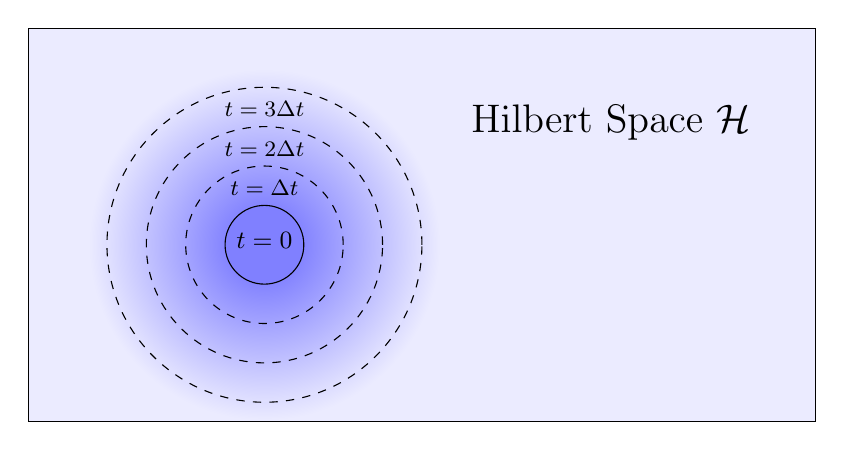
\begin{tikzpicture}[inner sep=1mm]

\node[rectangle,draw=black,fill=blue!8,minimum height=5cm,minimum width=10cm] (H) at (0,0) {};


\shade[inner color=blue!60,outer color=blue!8] (-2,-0.25) circle [radius=2.22cm];
\shade[inner color=blue!60,outer color=blue!12] (-2,-0.25) circle [radius=2cm];

\draw[radius=1.0,draw=black,dashed] (-2,-0.25) circle;
\draw[radius=1.5,draw=black,dashed] (-2,-0.25) circle;
\draw[radius=2.0,draw=black,dashed] (-2,-0.25) circle;

\filldraw[radius=0.5,draw=black,fill=blue!50] (-2,-0.25) circle;

\node (H1) at (2.4,1.3) {\Large Hilbert Space $\mathcal{H}$};
\node (t0) at (-2,-0.2) {\small $t = 0$};
\node (t1) at (-2,0.47) {\footnotesize $t = \Delta t$};
\node (t2) at (-2,0.97) {\footnotesize $t = 2 \Delta t$};
\node (t3) at (-2,1.47) {\footnotesize $t = 3 \Delta t$};

\end{tikzpicture}
	\caption{Illustration of area law states and their time evolution. Ground states following area laws occupy a tiny corner of the many-body Hilbert space, which is drawn as the inner circle ($t = 0$). As such a state is evolved, it will continue to follow an area law for longer longer, although the number of contributing eigenstates will increase. which is illustrated by the growing area. }
	\label{fig:HilbertSpace}
\end{figure}


\section{Variational Ground State Search}
For large systems exact diagonalization of the Hamiltonian is impossible, whereby one must resort to variational methods in order to find ground states. A variational search involves finding the state, $\ket{\psi}$, which minimizes
\begin{equation}
	E = \frac{\bra{\psi} \hat{H} \ket{\psi}}{\braket{\psi | \psi}} \; .
	\label{eq:variational}
\end{equation}
The Hamiltonian must be expressed as a matrix product operator to be applied to the state. An example is given in Appendix \ref{chap:buildMPO}, where the Bose-Hubbard Hamiltonian is formulated through tensors. Furthermore, in a variational search the state is repeatedly modified until the expectation value of the Hamiltonian is minimized. Therefore, the tensor network corresponding to eq. \ref{eq:variational} must be contracted efficiently in order for the search to be viable.


\subsection{Efficient Application of a Hamiltonian to an MPS}
Section \ref{sec:MPO} detailed the application of a matrix product operator to a state, however, even further reductions to the computational cost are needed, as the overlap with the Hamiltonian is evaluated many times during the ground state search. The DMRG variational search algorithm updates only a single tensor of the state at a time, whereby most of the tensor network describing the operator overlap remains constant. Hence, most of the network can be stored and used for multiple calculations, which is one of the key properties of the DMRG algorithm.\\ 
Consider a matrix product state in a mixed-canonical form
\begin{align}
	\ket{\psi} &= \sum_{\boldsymbol{j}} A^{j_1} \ldots A^{j_{n-1}} \Psi^{j_n} B^{j_{n+1}} \ldots B^{j_{L}} \ket{\boldsymbol{j}} \nonumber \\
	&= \sum_{\alpha_{n-1} , \alpha_{n}} \Psi_{\alpha_{n-1} , \alpha_{n}}^{j_n} \ket{\alpha_{n-1}}_A \ket{j_n}  \ket{\alpha_{n}}_L \; ,
	\label{eq:MPSmixedsingle}
\end{align}
where $\Psi^{j_n}$ are the matrices of the central site, and $\ket{\alpha_{n-1}}_A$ and $\ket{\alpha_{n}}_B$ are block states introduced in eq. \eqref{eq:mixedA} and \eqref{eq:mixedB} respectively. In the basis $\{ \ket{\alpha_{n-1} }  , \; \ket{ j_n }  , \; \ket{\alpha_{n} } \}$ the individual matrix elements of the Hamiltonian can be expressed as
\begin{equation}
	\bra{\alpha_{n-1} j_n \alpha_{n}} \hat{H} \ket{\alpha_{n-1} ' j_n ' \alpha_{n} '} = \sum_{\boldsymbol{j} , \boldsymbol{j'}}  W^{j_1 , j_1 '} \ldots W^{j_L , j_L '}  \braket{\alpha_{n-1} j_n \alpha_{n} | \boldsymbol{j}} \braket{\boldsymbol{j'} | \alpha_{n-1} ' j_n ' \alpha_{n} '} \; , 
	\label{eq:HamiltonianMatrixElement}
\end{equation}
Where the $W$'s are the matrices of the Hamiltonian MPO.
Since the basis of local states $\{ \ket{\boldsymbol{j}} \}$ shares a state with the basis $\{ \ket{\alpha_{n-1} }  , \; \ket{ j_n }  , \; \ket{\alpha_{n} } \}$, eq. \eqref{eq:HamiltonianMatrixElement} can be re-written using $\sum_{\boldsymbol{j}} \braket{j_n | \boldsymbol{j}} = \sum_{\boldsymbol{j *}} \ket{ \boldsymbol{j *}}$, where "$\boldsymbol{j *}$" means "excluding $j_n$". Thus,
\begin{align}
&	\bra{\alpha_{n-1} j_n \alpha_{n}} \hat{H} \ket{\alpha_{n-1} ' j_n ' \alpha_{n} '} = \nonumber \\
 &= \sum_{\boldsymbol{j *} , \boldsymbol{j' * }}  W^{j_1 , j_1 '} \ldots W^{j_n , j_n '} \ldots W^{j_L , j_L '} \nonumber \\
	& \qquad \times \braket{\alpha_{n-1} | j_1 \ldots j_{n-1}} \braket{\alpha_{n} | j_{n+1} \ldots j_{L}} \braket{j_1 ' \ldots j_{n-1} ' | \alpha_{n-1} '} \braket{j_{n+1} ' \ldots j_{L} ' | \alpha_{n} '} \nonumber \\
	&= \sum_{\boldsymbol{j *} , \boldsymbol{j' * }}  W^{j_1 , j_1 '} \ldots W^{j_n , j_n '} \ldots W^{j_L , j_L '} \nonumber \\
	& \qquad \times \left( A^{j_1} \ldots A^{j_{n-1}} \right)_{1 , \alpha_{n-1}}^{*} \left( B^{j_{n+1}} \ldots B^{j_{L}} \right)_{ \alpha_{n} , 1}^{*} \left( A^{j_1 '} \ldots A^{j_{n-1} '} \right)_{1 , \alpha_{n-1} '} \left( B^{j_{n+1} '} \ldots B^{j_{L} '} \right)_{ \alpha_{n} ' , 1} \nonumber \\
	&= \sum_{\alpha_n , \beta_n , \alpha_n '}
	\left( \sum_{j_1 , j_1 '} A_{1 , \alpha_1}^{j_1 *} W_{1, \beta_1}^{j_1 , j_1 '} A_{1 , \alpha_1 '}^{j_1 '} \right)
	\left( \sum_{j_2 , j_2 '} A_{\alpha_1 , \alpha_2}^{j_2 *} W_{\beta_1, \beta_2}^{j_2 , j_2 '} A_{\alpha_1 ' , \alpha_2 '}^{j_2 '} \right)
	\ldots W_{\beta_{n_1}, \beta_n}^{j_n , j_n '} \nonumber \\
	& \qquad \times \left( \sum_{j_{n+1} , j_{n+1} '} B_{\alpha_n , \alpha_{n+1}}^{j_{n+1} *} W_{\beta_n, \beta_{n+1}}^{j_{n+1} , j_{n+1} '} B_{\alpha_n ', \alpha_{n+1} '}^{j_{n+1} '} \right)
	\left( \sum_{j_{L} , j_{L} '} B_{\alpha_{L-1} , 1}^{j_{L} *} W_{\beta_{L-1}, 1}^{j_{L} , j_{L} '} B_{\alpha_{L-1}' , 1 }^{j_{L} '} \right)  \; .
\end{align}  
While this expression may seem terrible complicated due to all the indices, it is actually rather easy to understand. First, the matrix element is written excluding the local basis states $\ket{j_n}$. Next, the Hamilton MPO is projected into the block states of A, $\ket{\alpha_{n-1}}_A$, and B, $\ket{\alpha_{n}}_B$. Finally, the matrices are grouped according to their expansion in the local basis. Working with the above expression appears cumbersome, but it is merely a decoupling of the system into three distinct parts, which can be seen in figure \ref{fig:singleElemHamil}.
\begin{figure}[b!]
	\centering
	\begin{tikzpicture}[inner sep=1mm]
    \foreach \i in {1,...,4} {
        \node[tensorl] (tt\i) at (2* \i -1, 0) {};
        \node[operator] (o\i) at (2* \i -1, -1.5) {};
        \node[tensorl] (tb\i) at (2* \i -1, -3) {};
        
        
        \draw[-] (tt\i) -- (o\i);
        \draw[-] (o\i) -- (tb\i);
    };
    \foreach \i in {6,...,7} {
        \node[tensorr] (tt\i) at (2* \i -1, 0) {};
        \node[operator] (o\i) at (2* \i -1, -1.5) {};
        \node[tensorr] (tb\i) at (2* \i -1, -3) {};
        
        
        \draw[-] (tt\i) -- (o\i);
        \draw[-] (o\i) -- (tb\i);
    };
        \foreach \i in {1,...,3} {
        \pgfmathtruncatemacro{\iplusone}{\i + 1};
        \draw[-] (tt\i) -- (tt\iplusone);
        \draw[-] (tb\i) -- (tb\iplusone);
        \draw[-] (o\i) -- (o\iplusone);
    };
    \draw[-] (tt6) -- (tt7);
    \draw[-] (tb6) -- (tb7);
    \draw[-] (o6) -- (o7);
    
    
       
	\node[operator] (o5) at (2* 5 -1, -1.5) {};    
    
    \node (a1) at (8,0.5) {$\alpha_{n-1}$};
    \node (a2) at (10,0.5) {$\alpha_{n}$};
    \node (a1p) at (8,-3.5) {$\alpha_{n-1} '$};
    \node (a2p) at (10,-3.5) {$\alpha_{n} '$};
    \node (j) at (9,-0.5) {$j_n$};
    \node (jp) at (9,-2.5) {$j_n '$};
    
    \node (a1d) at (8,0) {};
    \node (a2d) at (10,0) {};
    \node (a1pd) at (8,-3) {};
    \node (a2pd) at (10,-3) {};
    
    \draw[-] (tt4) -- (a1d);
    \draw[-] (tt6) -- (a2d);
    \draw[-] (tb4) -- (a1pd);
    \draw[-] (tb6) -- (a2pd);
    \draw[-] (o5) -- (j);
    \draw[-] (o5) -- (jp);
    \draw[-] (o5) -- (o4);
    \draw[-] (o5) -- (o6);
    
    \node (d1) at (8,-0.75) {};
    \node (d2) at (8,-2.25) {};
   	\draw[dashed] (d1) -- (d2);
   	\node (d3) at (10,-0.75) {};
    \node (d4) at (10,-2.25) {};
   	\draw[dashed] (d3) -- (d4);
   	
   	
   	\node (L) at (4,-4.5) {L};
   	\node (W) at (9,-4.5) {W};
   	\node (R) at (12,-4.5) {R};
\end{tikzpicture}
	\caption{Representation of the matrix element $\bra{\alpha_{n-1} j_n \alpha_{n}} \hat{H} \ket{\alpha_{n-1} ' j_n ' \alpha_{n} '}$ as an tensor network. The network can be factorize into three distinct parts: The left (L) and right (R) environments consisting of the contracted network to the left and right of the operator tensor, $W^{[n]}$, respectively.}
	\label{fig:singleElemHamil}
\end{figure}
Since both the left and right side of the network is connected, one can contract these parts into two separate tensors $L$ and $R$ called \textit{environments}:
\begin{align}
	L_{\alpha_{n}, \beta_{n} , \alpha_{n} '} &= \sum_{ \substack{ \{ \alpha_i \beta_i \alpha_i ' \} \\ i < n}} \left( \sum_{j_1 , j_1 '} A_{1 , \alpha_1}^{j_1 *} W_{1, \beta_1}^{j_1 , j_1 '} A_{1 , \alpha_1 '}^{j_1 '} \right) \ldots \left( \sum_{j_{n} , j_{n} '} A_{\alpha_{n-1} , \alpha_{n}}^{j_{n} *} W_{\beta_{n-1}, \beta_{n}}^{j_{n} , j_{n} '} A_{\alpha_{n-1} ' , \alpha_{n} '}^{j_{n} '} \right) \label{eq:Ltensor} \\
	R_{\alpha_{n} ,\beta_{n} , \alpha_{n} '} &= \sum_{ \substack{ \{ \alpha_i \beta_i \alpha_i ' \} \\ i > n}} \left( \sum_{j_{n+1}  j_{n+1} '} B_{\alpha_n , \alpha_{n+1}}^{j_{n+1} *} W_{\beta_n, \beta_{n+1}}^{j_{n+1} , j_{n+1} '} B_{\alpha_n ', \alpha_{n+1} '}^{j_{n+1} '} \right) \ldots \nonumber \\
	& \qquad \qquad \qquad \qquad \qquad \qquad \qquad \times \left( \sum_{j_{L} , j_{L} '} B_{\alpha_{L-1} , 1}^{j_{L} *} W_{\beta_{L-1}, 1}^{j_{L} , j_{L} '} B_{\alpha_{L-1}' , 1 }^{j_{L} '} \right) \label{eq:Rtensor}
\end{align}
From these contractions, the tripartite structure of the Hamiltonian matrix elements, as seen in figure \ref{fig:singleElemHamil}, can be written in a compact way
\begin{equation}
	\bra{\alpha_{n-1} j_n \alpha_{n}} \hat{H} \ket{\alpha_{n-1} ' j_n ' \alpha_{n} '} = \sum_{\beta_{n-1} , \beta_{n}} L_{\alpha_{n-1}, \beta_{n-1} , \alpha_{n-1} '} \; W_{\beta_{n_1}, \beta_n}^{j_n , j_n '} \; R_{\alpha_{n} ,\beta_{n} , \alpha_{n} '} \; .
\end{equation}
Finally, applying the Hamiltonian in the $\{ \ket{\alpha_{n-1} } \; , \; \ket{ j_n } \; , \; \ket{\alpha_{n} } \}$ basis to the MPS of eq. \eqref{eq:MPSmixedsingle} yields \cite{schollwock}
\begin{equation}
	\hat{H} \ket{\psi} = \sum_{\beta_{n-1} , \beta_{n}} \sum_{\alpha_{n-1}' , j_n ', \alpha_{n}'} L_{\alpha_{n-1}, \beta_{n-1} , \alpha_{n-1} '} \; W_{\beta_{n_1}, \beta_n}^{j_n , j_n '} \; R_{\alpha_{n} ,\beta_{n} , \alpha_{n} '} \; \Psi_{\alpha_{n-1} ' , \alpha_{n} '}^{j_n '} \ket{\alpha_{n-1}}_A \ket{j_n} \ket{\alpha_{n}}_B \; .
	\label{eq:HPsi}
\end{equation}
Expressing $\hat{H}$ in the basis of the block states exposes the central site of the MPS such that it can be varied in a ground state search. Evaluating $\hat{H} \ket{\psi}$ must be done many times during a variational search of the ground state, hence this operation must be executed as fast as possible. Examining eq. \eqref{eq:HPsi} one will notice that while the boundaries of $L$ and $R$ will change depending on which site is being optimized, the bulk of the two tensors remain constant through most of the calculations. Instead of calculating $L$ and $R$ from eq. \eqref{eq:Ltensor} and \eqref{eq:Rtensor} for every evaluation of eq. \eqref{eq:HPsi}, one can iteratively build them, since they only change by one column of the network at a time. Thus, a large number of computations can be reused.\\
Consider the construction of the tensor $L^{[i]}$, which can be built iteratively from the left by contracting the previous left-tensor $L^{[i-1]}$ with the i'th column of the network consisting of $A^{[i]}$, $W^{[i]}$ and $A^{[i] \dag}$
\begin{equation}
	L_{\alpha_i , \beta_i , \alpha_i '}^{[i]} = \sum_{\substack{ j_i , j_i ' \\ \alpha_{i-1} , \beta_{i-1} , \alpha_{i-1} '}} W_{\beta_{i-1} , \beta_i}^{[i] j_i , j_i '} \left( A^{[i] j_i \dag} \right)_{\alpha_i , \alpha_{i-1}} L_{\alpha_{i-1} , \beta_{i-1} , \alpha_{i-1} '}^{[i-1]} A_{\alpha_{i-1} ' , \alpha_i '}^{[i] j_i '} \; .
\end{equation}
The iterative update of $L^{[i]}$ can be seen illustrated in figure \ref{fig:buildLTensor}. The square-bracket notation has been re-introduced to keep track of the tensors relation to the physical sites. In order to remain consistent with notation, the dummy scalars $L_{\alpha_0 , \beta_0 , \alpha_0 '}^{[0]}  = 1  = \alpha_0 , \beta_0 , \alpha_0 '$ have been introduced.\\
\begin{figure}[h!]
	\centering
	\begin{tikzpicture}[inner sep=1mm]
	\def \numb {2};
	\def \hdist {1.5};
	\def \offset {6};

    \foreach \i in {1,...,\numb} {
        \node[tensorl] (tt\i) at (\i*\hdist, 0) {};
        \node[operator] (o\i) at (\i*\hdist, -1.5) {};
        \node[tensorl] (tb\i) at (\i*\hdist, -3) {};  
        
        \draw[-] (tt\i) -- (o\i);
        \draw[-] (o\i) -- (tb\i);
    };
    \foreach \i in {1,...,1} {
        \pgfmathtruncatemacro{\iplusone}{\i + 1};
        \draw[-] (tt\i) -- (tt\iplusone);
        \draw[-] (tb\i) -- (tb\iplusone);
        \draw[-] (o\i) -- (o\iplusone);
    };
    \foreach \i in {\offset,...,8} {
        \node[tensorl] (tt\i) at (\i*\hdist, 0) {};
        \node[operator] (o\i) at (\i*\hdist, -1.5) {};
        \node[tensorl] (tb\i) at (\i*\hdist, -3) {};  
        
        \draw[-] (tt\i) -- (o\i);
        \draw[-] (o\i) -- (tb\i);
    };
    \foreach \i in {\offset,...,7} {
        \pgfmathtruncatemacro{\iplusone}{\i + 1};
        \draw[-] (tt\i) -- (tt\iplusone);
        \draw[-] (tb\i) -- (tb\iplusone);
        \draw[-] (o\i) -- (o\iplusone);
    };
    
    \node[tensor] (tt) at (\numb*\hdist+1.5*\hdist, 0) {$U$};
    \node[operator] (o) at (\numb*\hdist+1.5*\hdist, -1.5) {};
    \node[tensor] (tb) at (\numb*\hdist+1.5*\hdist, -3) {$U^{\dag}$};

	\draw[-] (tt) -- (o);
	\draw[-] (tb) -- (o);
    
    \node (at1) at (\numb*\hdist+0.8*\hdist, 0) {$\alpha_{i-1}$};
    \node (at2) at (\numb*\hdist+2.25*\hdist, 0) {$\alpha_{i}$};
    \node (ab1) at (\numb*\hdist+0.8*\hdist, -3) {$\alpha_{i-1} '$};
    \node (ab2) at (\numb*\hdist+2.25*\hdist, -3) {$\alpha_{i} '$};
    \node (b1) at (\numb*\hdist+0.8*\hdist, -1.5) {$\beta_{i-1}$};
    \node (b2) at (\numb*\hdist+2.25*\hdist, -1.5) {$\beta_{i}$};
    
    \draw[-] (tt\numb) -- (at1);
    \draw[-] (tb\numb) -- (ab1);
    \draw[-] (o\numb) -- (b1);
    \draw[-] (tt) -- (at1);
    \draw[-] (tb) -- (ab1);
    \draw[-] (o) -- (b1);
    \draw[-] (tt) -- (at2);
    \draw[-] (tb) -- (ab2);
    \draw[-] (o) -- (b2);
    
    
    \draw[->, line width=1mm] (\numb*\hdist+2.65*\hdist,-1.5) -- (\numb*\hdist+3.55*\hdist,-1.5);
    
    \node (at3) at (\offset*\hdist+\numb*\hdist+0.8*\hdist, 0) {$\alpha_{i}$};
    \node (ab3) at (\offset*\hdist+\numb*\hdist+0.8*\hdist, -3) {$\alpha_{i} '$};
    \node (b3) at (\offset*\hdist+\numb*\hdist+0.8*\hdist, -1.5) {$\beta_{i}$};
    \draw[-] (tt8) -- (at3);
    \draw[-] (tb8) -- (ab3);
    \draw[-] (o8) -- (b3);
    
    \node (L1) at (2.5,-4) {$L^{[i-1]}$};
    \node (L2) at (\offset*\hdist+\hdist,-4) {$L^{[i]}$};

    
    \node (eq) at (\offset*\hdist+\numb*\hdist+1.35*\hdist,-1.5) {$\equiv$};
    

    \node (dummy1) at (\offset*\hdist+\numb*\hdist+2.8*\hdist,0) {$\alpha_{i}$};
 	\node (dummy2) at (\offset*\hdist+\numb*\hdist+2.8*\hdist,-3) {$\alpha_{i} '$};
 	\node (dummy3) at (\offset*\hdist+\numb*\hdist+2.8*\hdist,-1.5) {$\beta_{i}$};
	\node[tensor] (mat) at (\offset*\hdist+\numb*\hdist+2*\hdist , -1.5) {};    
    
    \draw[-] (dummy1.west) .. controls (\offset*\hdist+\numb*\hdist+2*\hdist, 0) .. (mat.north);
    \draw[-] (dummy2.west) .. controls (\offset*\hdist+\numb*\hdist+2*\hdist, -3) .. (mat.south);
	\draw[-] (mat) -- (dummy3);   
	
	
	\node (L3) at (\offset*\hdist+\numb*\hdist+2.25*\hdist,-4) {$L^{[i]}$}; 
\end{tikzpicture}
	\caption{\textit{Iterative update from $L^{[i-1]}$ to $L^{[i]}$ through a contraction of $L^{[i-1]}$ with $A^{[i]}$, $W^{[i]}$ and $A^{[i] \dag}$. The result is a tensor with three horizontal legs.}}
	\label{fig:buildLTensor}
\end{figure}
It is important to store every iteration of $L^{[i]}$, since $L$ will grow and shrink constantly throughout the variational search of the ground state, whereby every iteration of $L^{[i]}$ will be used multiple times.
The same applies when building the right environment, $R$. Here one starts from the right and moves left when iteratively contracting the tensor. Applying optimal bracketing, the cost of updating the environments scales as $\mathcal{O}(d D^3 D_W)$.
  

\subsection{Iterative Ground State Search and the DMRG Algorithm} \label{sec:DMRG}
In order to find the ground state of the system on can introduce a Lagrangian multiplier, $\lambda$, and extremize
\begin{equation}
	\bra{\psi} \hat{H} \ket{\psi} - \lambda \braket{\psi | \psi} \; ,
	\label{eq:lagrange}
\end{equation}
whereby the desired ground state, $\ket{\psi}$, and ground state energy, $\lambda^0$, will be reached.\\
Trying to optimize an entire MPS at once is a highly non-linear problem involving an extremely large number of variables. However, the problem can be linearised by only considering the variables of a single tensor (site) at a time, while keeping the rest of the MPS constant. By varying just a single tensor at a time, one will continuously find states lower in energy, until convergence is reached. However, this procedure is very prone to getting stuck in a local extrema. To circumvent this, one can consider two sites at a time and optimize with regards to a two-site tensor, created by momentarily merging the two sites \cite{White1993}.

Consider the variation of the tensors $M^{[n]}$ and $M^{[n+1]}$. Expressing the minimization problem of eq. \eqref{eq:lagrange} in terms of the left and right environments (as done in eq. \eqref{eq:HPsi}) yields
\begin{align}
	\bra{\psi} \hat{H} \ket{\psi} &= \sum_{\substack{j_n , j_n ' \\ j_{n+1} , j_{n+1} '}} \sum_{\alpha_{n-1} ' , \alpha_n ', \alpha_{n+1} '} \sum_{\alpha_{n-1} , \alpha_n , \alpha_{n+1}} \sum_{\beta_{n-1} , \beta_n , \beta_{n+1}} L_{\alpha_{n-1}, \beta_{n-1} , \alpha_{n-1} '}^{[n-1]} \; W_{\beta_{n_1}, \beta_n}^{j_n , j_n '} \; W_{\beta_{n}, \beta_{n+1}}^{ j_{n+1} , j_{n+1} '} \nonumber \\
	& \qquad \times R_{\alpha_{n+1} ,\beta_{n+1} , \alpha_{n+1} '}^{[n+2]} \; M_{\alpha_{n-1} , \alpha_{n}}^{j_n } \; M_{\alpha_{n-1} ' , \alpha_{n} '}^{j_n ' *} \; M_{\alpha_{n} , \alpha_{n+1}}^{j_{n+1} } \; M_{\alpha_{n} ' , \alpha_{n+1} '}^{j_{n+1} ' *}  \label{eq:twositeHamil}
\end{align}
with the overlap
\begin{align}
	\braket{\psi | \psi} &= \sum_{j_n , j_{n+1} } \sum_{\substack{\alpha_{n-1} ' \\ \alpha_n ', \alpha_{n+1} '}} \sum_{\alpha_{n-1} , \alpha_n ,\alpha_{n+1}} \Psi_{\alpha_{n-1},\alpha_{n-1}'}^{A} \; M_{\alpha_{n-1} , \alpha_{n}}^{ j_n } \; M_{\alpha_{n-1} ' , \alpha_{n} '}^{j_n ' *} \nonumber \\
	& \qquad \times M_{\alpha_{n} , \alpha_{n+1}}^{j_{n+1} } \; M_{\alpha_{n} ' , \alpha_{n+1} '}^{j_{n+1} ' *} \; \Psi_{\alpha_{n+1},\alpha_{n+1}'}^{B} \; , \label{eq:twositeOverlap}
\end{align}
where the Hamiltonian from eq. \eqref{eq:HPsi} has been re-ordered to accommodate examining two sites, $n$ and $n+1$, at a time, and 
\begin{align}
\Psi_{\alpha_{n-1},\alpha_{n-1}'}^{A} &= \sum_{j_1 , \ldots , j_{n-1}} \left( M^{j_{n-1} \dag} \ldots M^{j_{1} \dag} M^{j_1} \ldots M^{j_{n-1}} \right) _{\alpha_{n-1} , \alpha_{n-1} '} \label{eq:psiA} \\
\Psi_{\alpha_{n+1},\alpha_{n+1}'}^{B} &= \sum_{j_{n+2} , \ldots , j_{L}} \left( M^{j_{n+2} } \ldots M^{j_{L} } M^{j_L \dag} \ldots M^{j_{n+2} \dag} \right) _{\alpha_{n+1} ', \alpha_{n+1} } \; .
\end{align}
Further simplifications can be made for mixed-canonical forms, if sites $1$ through $n-1$ are left-normalized, and sites $n+2$ through $L$ are right-normalized, whereby
\begin{equation}
	\Psi_{\alpha_{n-1},\alpha_{n-1}'}^{A} = \delta_{\alpha_{n-1},\alpha_{n-1}'} \qquad , \qquad \Psi_{\alpha_{n+1},\alpha_{n+1}'}^{B} = \delta_{\alpha_{n+1},\alpha_{n+1}'} \; .
\end{equation}
Finding the extremum of eq. \eqref{eq:lagrange} with respect to $M_{\alpha_{n-1} ' , \alpha_{n} '}^{[n] j_n ' } \; M_{\alpha_{n} ' , \alpha_{n+1} '}^{[n+1] j_{n+1} ' }$ is done through the following sequence:

\subsubsection{Two-site update for iterative ground state search}
\begin{enumerate}
\item
\textbf{Merge:} Contract the two matrices $M^{[n]}$ and $M^{[n+1]}$ over the bond $\alpha_{n}$ creating a two-site tensor
\begin{equation}
\Theta_{\alpha_{n-1} , \alpha_{n+1}}^{j_n , j_{n+1}} = \sum_{\alpha_n} M_{\alpha_{n-1} , \alpha_{n}}^{[n] j_n } \;  M_{\alpha_{n} , \alpha_{n+1}}^{[n+1] j_{n+1} } 
\end{equation}

\item
\textbf{Solve eigenproblem:} This yields an eigenvalue problem, which can be seen by reshaping
\begin{align}
	H_{( \alpha_{n-1}  j_n  j_{n+1}, \alpha_{n+1}),(\alpha_{n-1}'  j_n '  j_{n+1}', \alpha_{n+1}')} &= \nonumber \\
	= \; \sum_{\substack{\beta_{n-1} , \beta_n \\ \beta_{n+1}}} L_{\alpha_{n-1}, \beta_{n-1} , \alpha_{n-1} '}^{[n-1]} & \; W_{\beta_{n_1}, \beta_n}^{[n] j_n , j_n '} \; W_{\beta_{n}, \beta_{n+1}}^{[n+1] j_{n+1} , j_{n+1} '}\;  R_{\alpha_{n+1} ,\beta_{n+1} , \alpha_{n+1} '}^{[n+2]} 
\end{align}
and
\begin{equation}
	v_{ \alpha_{n-1} j_n j_{n+1} \alpha_{n+1}} = \; \Theta_{\alpha_{n-1} , \alpha_{n+1}}^{j_n , j_{n+1}}
\end{equation}
such that
\begin{equation}
	H v - \lambda v = 0 \; .
	\label{eq:eigprob}
\end{equation}
Solving eq. \eqref{eq:eigprob} for the lowest eigenvalue $\lambda_0$ yields $v_{ \alpha_{n-1} j_n j_{n+1} \alpha_{n+1}}^0$, which can be reshaped back to the now optimized two-site tensor, $\tilde{\Theta}_{\alpha_{n-1} , \alpha_{n+1}}^{j_n , j_{n+1}}$.

\item
\textbf{Unmerge:} Reshape the updated $\tilde{\Theta}_{\alpha_{n-1} , \alpha_{n+1}}^{j_n , j_{n+1}}$ to a matrix and perform an SVD yielding
\begin{equation}
	\tilde{\Theta}_{(j_n \alpha_{n-1} ) ,(j_{n+1}  \alpha_{n+1} )} = \sum_{\alpha_n} U_{\alpha_{n-1} , \alpha_{n}}^{j_n} S_{\alpha_n , \alpha_n} (V^{\dag})_{\alpha_{n} , \alpha_{n+1}}^{j_{n+1}} \; .
\end{equation}
This causes the bond dimension to increase $D \rightarrow d D$, which must be truncated by keeping only the $D$ largest singular values of $S$. 

\item
\textbf{Update environments:} The last step depends on which direction, one is iterating trough the chain. Here, the left- and right-normalization of $U$ and $V^{\dag}$ is used to update the environments.\\
\textit{Going right}: Update the left environment
\begin{equation}
	\tilde{L}_{\alpha_{n}, \beta_{n} , \alpha_{n} '}^{[n]} = \sum_{\substack{ j_{n} , j_{n} ' \\ \alpha_{n-1} , \beta_{n-1} , \alpha_{n-1} '}} L_{\alpha_{n-1}, \beta_{n-1} , \alpha_{n-1} '}^{[n-1]} \; U_{\alpha_{n-1} , \alpha_{n}}^{j_n} \; W_{\beta_{n-1} , \beta_{n}}^{[n] j_n , j_n '} \; U_{\alpha_{n-1} ', \alpha_{n}'}^{j_n ' *} \; ,
\label{eq:updateLeft}
\end{equation}
and build the matrix of the right site
\begin{equation}
	\tilde{M}_{\alpha_{n} , \alpha_{n+1}}^{[n+1] j_{n+1} } = \sum_{\alpha_n}  S_{\alpha_n , \alpha_n} (V^{\dag})_{\alpha_{n} , \alpha_{n+1}}^{j_{n+1}} \; .
\end{equation}\\ 
\textit{Going left}: Update the right environment
\begin{equation}
	\tilde{R}_{\alpha_{n}, \beta_{n} , \alpha_{n} '}^{[n+1]} = \sum_{\substack{ j_{n+1} , j_{n+1} ' \\ \alpha_{n+1} , \beta_{n+1} , \alpha_{n+1} '}} R_{\alpha_{n+1}, \beta_{n+1} , \alpha_{n+1} '}^{[n+2]} \; \left( V^{\dag} \right)_{\alpha_{n} , \alpha_{n+1}}^{j_{n+1}} \; W_{\beta_{n} , \beta_{n+1}}^{[n+1] j_{n+1} , j_{n+1} '} \; \left( V^{\dag} \right)_{\alpha_{n} , \alpha_{n+1}}^{j_{n+1} *} \; ,
	\label{eq:updateRight}
\end{equation}
and build the matrix of the left site
\begin{equation}
	\tilde{M}_{\alpha_{n-1} , \alpha_{n}}^{[n] j_{n} } = \sum_{\alpha_n} U_{\alpha_{n-1} , \alpha_{n}}^{j_n} S_{\alpha_n , \alpha_n}  \; .
\end{equation} 
 
\end{enumerate}
This concludes the two-site update sequence, which is illustrated in figure \ref{fig:twoSiteUpdate}. After performing the sequence, one can move \textit{one site} to either left or right, depending on which direction one is iterating.

\renewcommand{\thesubfigure}{\arabic{subfigure}}
\begin{figure}[h!]
	\centering
	\begin{subfigure}{\textwidth}
		\centering
		\caption{\textbf{Merge:}}
		\begin{tikzpicture}[inner sep=1mm]
	\def \imgcenter {5.25};
	\def \imgwidth {15};
	\node[minimum width=\imgwidth cm] (fake) at (\imgcenter ,0) {};


    \node[tensor] (M1) at (1 , 0) {};
    \node[tensor] (M2) at (2.5 , 0) {};
	\node[tensor, minimum width=2cm] (sig) at (9, 0) {};
	
	\node (j1) at (1 ,-1) {$j_n$};
	\node (j2) at (2.5 ,-1) {$j_{n+1}$};
	\node (a1) at (-0.2 ,0) {$\alpha_{n-1}$};
	\node (a2) at (3.7 ,0) {$\alpha_{n+1}$};    
    
	\draw[-] (M1) -- (j1);
	\draw[-] (M1) -- (a1);
	\draw[-] (M1) -- (M2);
	\draw[-] (M2) -- (j2);
	\draw[-] (M2) -- (a2);
	
	
	\node (node1) at (8.35, -1) {$j_n$};
	\node (node2) at (9.65, -1) {$j_{n+1}$};
	\node (as1) at (7 ,0) {$\alpha_{n-1}$};
	\node (as2) at (11 ,0) {$\alpha_{n+1}$};
	
	\draw[-] (node1) -- (node1 |-  sig.south);
	\draw[-] (node2) -- (node2 |-  sig.south);
	\draw[-] (sig) -- (as1);
	\draw[-] (sig) -- (as2);		
	
	\draw[->, line width=1mm] (4.5,0) -- (6,0);
	
	\node (Mlab1) at (1,0.8) {$M^{[n]}$};
	\node (Mlab2) at (2.5,0.8) {$M^{[n+1]}$};
	\node (Siglab) at (9,0.7) {$\Theta$};
	
	
\end{tikzpicture}
	\end{subfigure}\\[.25cm]
	
	\begin{subfigure}{\textwidth}
		\centering
		\caption{\textbf{Solve eigenprobem:}}
		\begin{tikzpicture}[inner sep=1mm]
	\def \imgcenter {5.8};
	\def \imgwidth {15};
	\node[minimum width=\imgwidth cm] (fake) at (\imgcenter ,0) {};	
	
	
	\node[tensor, minimum width=2.5cm] (theta) at (2, 0) {};
	\node[operator] (W1) at (1.1,-1.5) {};
	\node[operator] (W2) at (2.9,-1.5) {};	
	
	\node (dummy1) at (0.3,-3) {};
 	\node (dummy2) at (3.6,-3) {};
	\node[tensor] (L) at (-0.5 , -1.5) {};
	\node[tensor] (R) at (4.5 , -1.5) {};    
    
    \draw[-] (dummy1.west) .. controls (-0.5, -3) .. (L.south);
    \draw[-] (dummy2.east) .. controls (4.5, -3) .. (R.south);
    \draw[-] (theta.west) .. controls (-0.5, 0) .. (L.north);
    \draw[-] (theta.east) .. controls (4.5, 0) .. (R.north);
	
	\draw[-] (L) -- (W1);
	\draw[-] (W1) -- (W2);
	\draw[-] (W2) -- (R);
	\draw[-] (W1) -- (W1 |-  theta.south);
	\draw[-] (W2) -- (W2 |-  theta.south);
	
	\node (j1) at (1.1 , -2.5) {$j_{n}'$};
	\node (j2) at (2.9 , -2.5) {$j_{n+1}'$};
	\draw[-] (W1) -- (j1);
	\draw[-] (W2) -- (j2);
	
	\node (a1) at (0.5 , -3.3) {$\alpha_{n-1}'$};
	\node (a2) at (3.6 , -3.3) {$\alpha_{n+1}'$};
	\node (Llab) at (-1.2 , -1.5) {$L$};
	\node (Rlab) at (5 , -1.6) {$R$};	
	\node (Thetalab) at (2 , 0.6) {$\tilde{\Theta}$};
	\node (W1lab) at (0.6 , -0.9) {$W^{[n]}$};
	\node (W2lab) at (3.6 , -0.9) {$W^{[n+1]}$};
	
	
	\def \offsetx {7.5};
	\def \offsety {-1};
	\node[tensor, minimum width=2.5cm] (theta2) at (2+\offsetx, \offsety) {};
	\node (d1) at (1.1 +\offsetx, -1+ \offsety) {};
	\node (d2) at (2.9 +\offsetx, -1 + \offsety) {};
	\node (d3) at (2+\offsetx - 1.25 - 0.8, 0+\offsety) {};
	\node (d4) at (2+\offsetx + 1.25 + 0.8, 0+\offsety) {};
	
	\draw[-] (d1) -- (d1 |-  theta2.south);
	\draw[-] (d2) -- (d2 |-  theta2.south);
	\draw[-] (d3) -- (theta2);
	\draw[-] (d4) -- (theta2);
	
	\node (Thetalab2) at (2 +\offsetx, 0.6 + \offsety) {$\tilde{\Theta}$};
	
	
	\node (eq) at (5.8 , -1.5) {$=$};
	\node (lambda) at (7 , -1.5) {$\lambda_0 \;  \times$};	
\end{tikzpicture}
	\end{subfigure}\\[.25cm]

	\begin{subfigure}{\textwidth}
		\centering
		\caption{\textbf{Unmerge:}}
		\begin{tikzpicture}[inner sep=1mm]	
	\def \center {2};
	\def \width {2.5};
	\def \offsetx {8};
	\def \xspace {1};
	\def \imgcenter {\offsetx -2.75};
	\def \imgwidth {15};
	\node[minimum width=\imgwidth cm] (fake) at (\imgcenter ,0) {};
	
	
	\node[tensor, minimum width=\width cm] (theta) at (\center, 0) {};
	
	\node (d1) at (\center - \width/2 + 0.35,-1) {};
	\node (d2) at (\center + \width/2 - 0.35,-1) {};
	\node (d3) at (\center - \width/2 - 0.8, 0) {};
	\node (d4) at (\center + \width/2 + 0.8, 0) {};
	
	\draw[-] (d1) -- (d1 |-  theta.south);
	\draw[-] (d2) -- (d2 |-  theta.south);
	\draw[-] (d3) -- (theta);
	\draw[-] (d4) -- (theta);	
	
	\node (thetalab) at (\center , 0 + 0.6) {$\tilde{\Theta}$};
	
	
	\node[tensor] (U) at (\offsetx , 0) {};
	\node[matrix] (S) at (\offsetx + \xspace, 0) {};
    \node[tensor] (V) at (\offsetx + 2*\xspace , 0) {};
	
	
	\node (j1) at (\offsetx ,-1) {$j_n$};
	\node (j2) at (\offsetx + 2*\xspace ,-1) {$j_{n+1}$};
	\node (a1) at (\offsetx -1.2 ,0) {$\alpha_{n-1}$};
	\node (a2) at (\offsetx + 2*\xspace +1.2 ,0) {$\alpha_{n+1}$};    
    
	\node (Ulab) at (\offsetx , 0.6) {$U$};
	\node (Slab) at (\offsetx + \xspace , 0.6) {$S$};
	\node (Vlab) at (\offsetx + 2*\xspace , 0.6) {$V^{\dag}$};    
    
	\draw[-] (U) -- (j1);
	\draw[-] (U) -- (a1);
	\draw[-] (U) -- (S);
	\draw[-] (V) -- (S);
	\draw[-] (V) -- (j2);
	\draw[-] (V) -- (a2);
	
	\draw[->, line width=1mm] (\offsetx-3.5 ,0) -- (\offsetx-2,0);
	\node (SVD) at (\offsetx-2.9 ,0.4) {SVD};
\end{tikzpicture}
	\end{subfigure}\\[.25cm]

	\begin{subfigure}{\textwidth}
		\centering
		\caption{\textbf{Update environments:}}
		\begin{tikzpicture}[inner sep=1mm]
	\def \offsetx {6};
	\def \offsety {-5};
	\def \imgcenter {\offsetx -2.25};
	\def \imgwidth {15};
	\node[minimum width=\imgwidth cm] (fake) at (\imgcenter ,0) {};
	

	\Left{-0.5}{-1.5}{1.5};
	\node[tensor] (U1) at (1,0) {};	
	\node[tensor] (U2) at (1,-3) {};	
	\node[operator] (W) at (1,-1.5) {};

	\node (a1) at (2,0) {$\alpha_n$};
	\node (a2) at (2,-3) {$\alpha_n '$};
	\node (b) at (2,-1.5) {$\beta_n$};
	
	\draw[-] (U1) -- (W);
	\draw[-] (U2) -- (W);
	\draw[-] (U1) -- (a1);
	\draw[-] (U2) -- (a2);
	\draw[-] (W) -- (b);
	
	\node (L1) at (-1.4,-1.5) {$L^{[n-1]}$};
	\node (U1lab) at (1,0.6) {$U$};
	\node (U2lab) at (1,-3.6) {$U^{\dag}$};
	
	
	\draw[->, line width=1mm] (\offsetx-3 ,-1.5) -- (\offsetx-1.5,-1.5);
	
	
	\Left{\offsetx}{-1.5}{1.2};
	\node (L2) at (\offsetx -0.8,-1.5) {$\tilde{L}^{[n]}$};
	\node (a1) at (\offsetx+1.5,0) {$\alpha_n$};
	\node (a2) at (\offsetx+1.5,-3) {$\alpha_n '$};
	\node (b) at (\offsetx+1.5,-1.5) {$\beta_n$};
	
	%%----------------%%
	
	\Right{1}{-1.5 + \offsety}{1.5};
	\node[tensor] (U1) at (-0.5,0 + \offsety) {};	
	\node[tensor] (U2) at (-0.5,-3 + \offsety) {};	
	\node[operator] (W) at (-0.5,-1.5 + \offsety) {};

	\node (a1) at (-1.8,0 + \offsety) {$\alpha_{n}$};
	\node (a2) at (-1.8,-3 + \offsety) {$\alpha_{n} '$};
	\node (b) at (-1.8,-1.5 + \offsety) {$\beta_{n}$};
	
	\draw[-] (U1) -- (W);
	\draw[-] (U2) -- (W);
	\draw[-] (U1) -- (a1);
	\draw[-] (U2) -- (a2);
	\draw[-] (W) -- (b);
	
	\node (R1) at (2,-1.5 + \offsety) {$R^{[n+2]}$};
	\node (V1lab) at (-0.5,0.6 + \offsety) {$V^{\dag}$};
	\node (V2lab) at (-0.5,-3.6 + \offsety) {$V$};
	
	
	\draw[->, line width=1mm] (\offsetx-3 ,-1.5 + \offsety) -- (\offsetx-1.5,-1.5 + \offsety);
	
	
	\Right{\offsetx + 1.2}{-1.5 + \offsety}{1.2};
	\node (R2) at (\offsetx +2.2,-1.5 + \offsety) {$\tilde{R}^{[n+1]}$};
	\node (a1) at (\offsetx -0.5,0 + \offsety) {$\alpha_{n}$};
	\node (a2) at (\offsetx -0.5,-3 + \offsety) {$\alpha_{n} '$};
	\node (b) at (\offsetx -0.5,-1.5 + \offsety) {$\beta_{n}$};
\end{tikzpicture}
	\end{subfigure}
	
	
	\caption{\textit{Diagrammatic representation of the two-site update sequence for iterative ground state search. Step \textbf{(2)} optimizes with regard to two sites, but only a single site is updated to avoid getting stuck. In step \textbf{(4)}, when iterating left-to-right in the lattice, the left environment, $L^{[n]}$, is updated. The right environment, $R^{[n]}$, is updated when moving right-to-left.}}
	\label{fig:twoSiteUpdate}
\end{figure}

Some comments regarding the sequence are in order: The matrices of the eigenvalue problem have dimensions $( d^2 D^2 \times d^2 D^2)$, which is generally too much for exact diagonalization, however, since only the lowest eigenvalue is of interest, one can use an iterative eigensolver \cite{Lanczos}. Furthermore, if the MPS is not in the proper mixed-canonical form, the eigenvalue problem turns into a generalized eigenvalue problem, which can be numerically quite demanding. Thus, updating the left and right environments in step (4) is necessary, since it leads to great simplifications in step (2). Lastly, one could also consider just a single site when updating, however, this method is very prone to getting stuck \cite{White2005}. By updating two sites at once, one actually optimizes the bond between them. Hence, after updating the two sites, one must only iterate a single site. Optimization is done with regards to the current configuration, whereby it depends on previous updates. To compensate for this, one must sweep through the entire system multiple times, which leads to the basic DMRG algorithm shown below.
\begin{algorithm}[!h]
\begin{algorithmic}
\caption{Iterative ground state search (DMRG)}
\State Choose $\ket{\psi}$ right-normalized.
\State Calculate tensor $R^{[i]}$ iteratively for $i = L \ldots 1$.
\While{Stopping criteria not met} 
	\For{$n = 1 \ldots L-1$} \Comment{Left sweep}
		\State Perform two-site update on $M^{[n]}$ and $M^{[n+1]}$.
		\State Update $L^{[n]}$ according to eq. \eqref{eq:updateLeft}
	\EndFor
	\For{$n = L-1 \ldots 1$} \Comment{Right sweep}
		\State Perform two-site update on $M^{[n]}$ and $M^{[n+1]}$.
		\State Update $R^{[n]}$ according to eq. \eqref{eq:updateRight}
	\EndFor
\EndWhile
\end{algorithmic}
\end{algorithm}


\subsection{Applications of DMRG Algorithm on Bose-Hubbard Systems} \label{chap:CondFrac}
The DMRG algorithm has proven itself to be one of the most powerful methods for describing ground states in one-dimensional systems. This will be illustrated here by characterizing equilibrium properties of the Bose-Hubbard phases. First, the DMRG algorithm is compared to exact diagonalization methods applied on small systems, where the eigenstates of the Hamiltonian are extracted directly by diagonalizing the Hamilton matrix. Exact diagonalization is only applicable on small systems, due to the exponential scaling of the Hilbert space \cite{Vidal2003}. Referring back to eq. \eqref{eq:HilberSpaceScaling}, a Bose-Hubbard system with 10 sites and unit occupation has a Hilbert space dimension around $D_{\mathcal{H}}^{(L = 10)} = 9.2 \cdot 10^{4}$. The corresponding Hamiltonian matrix has a size of $D_{\mathcal{H}} \times D_{\mathcal{H}}$, although it is quite sparse, which enables sparse eigensolvers to find the ground state through exact diagonalization.
However, a 20-site Bose-Hubbard system will have a Hilbert space dimension of $D_{\mathcal{H}}^{(L = 20)} = 6.9 \cdot 10^{10}$, which is far outside the reach of exact diagonalization. Meanwhile, the DMGR algorithm can comfortably find very accurate ground states in such large Hilbert spaces. In fact, for the analysis presented here, systems up to 50 lattice sites are examined. Such systems have Hilbert spaces of astronomical dimensions $D_{\mathcal{H}}^{(L = 50)} = 5.0 \cdot 10^{28}$, however, as long as the ground state obeys an area law, the DMRG algorithm can easily find it in only a few sweeps through the lattice.


\subsubsection{Approximating the critical point through condensate fractions}

According to the Penrose-Onsager criterion, a system is in the superfluid phase if and only if the largest eigenvalue, $\lambda_1$, of the single-particle density matrix, $\rho^{(1)}$, is macroscopic
\begin{equation}
	f_c = \frac{\lambda_1}{N_p} > 0 \; ,
	\label{eq:condensateFraction}
\end{equation} 
where $f_c$ is the condensate fraction \cite{PenroseOnsager}. The entries of the density matrix are given by the single-particle correlations
\begin{equation}
	\rho_{i,j}^{(1)} = \bra{\psi} \hat{a}_{i}^{\dag} \hat{a}_{j} \ket{\psi} \; ,
	\label{eq:DensityMatrixEntry}
\end{equation}
where $\ket{\psi}$ is the ground state of the system. The ground state was found using both a version of the DMRG algorithm implemented in the ITensor library \cite{ITensor} and an exact diagonalization script used in \cite{MajaJulie}. If the state is parameterized through a tensor network, the correlations can be efficiently evaluated using the procedures detailed in Section \ref{sec:correlationFunctions}.

The condensate fraction can be used to determine which phase dominates the system, as
\begin{align}
	\lim_{N_p \to \infty} f_{c}^{\mathrm{SF}} &\to 1 \label{eq:SF_lim} \\
	\lim_{N_p \to \infty} f_{c}^{\mathrm{MI}} &\to 0 \; , \label{eq:MI_lim}
\end{align}
when the filling-fraction, $n = N_p/L$, is held constant. Thus, one should be able to recognize the phase of a Bose-Hubbard system at a given point $U/J$ through eq. \eqref{eq:SF_lim} and \eqref{eq:MI_lim}.
Therefore, the condensate fraction was calculated using ground state at various fractions $U/J$ for a series of system sizes. The results of this calculation are shown in figure \ref{fig:CondensateFraction}.
\begin{figure}[h!]
    \centering
    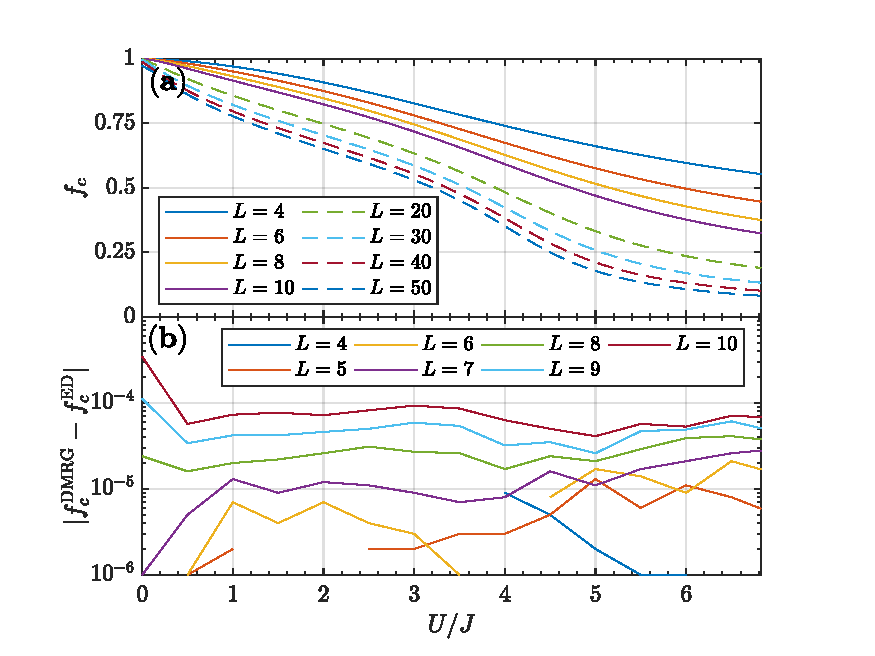
\includegraphics[width=0.9\textwidth]{Figures/CondensateFractionCompare.pdf}
 \caption{Condensate fraction of Bose-Hubbard system as function of $U/J$ for various system sizes. \textbf{(a)} Condensate fraction calculated using DMRG algorithm with a maximum bond dimension $D = 200$. The results were achieved through 5 DMRG sweeps, with exception of the $U/J \sim 0$ limit, where 20 sweeps were used. The dashed curves mark system sizes outside the scope of exact diagonalization. \textbf{(b)} Absolute difference between condensate fractions obtained through DMRG and exact diagonalization for small systems.}
 \label{fig:CondensateFraction}
\end{figure}

In order to confirm the accuracy of the DMRG algorithm, condensate fractions calculated for system sizes $L =  4 , \ldots , 10 $ were compared to results obtained through exact diagonalization, which can be seen in figure \ref{fig:CondensateFraction}(b). Clearly, the two methods produce very similar results when applied to small systems.

Meanwhile, figure \ref{fig:CondensateFraction}(a) displays the condensate fraction for various $U/J$ calculated using the DMRG algorithm. Although $f_c$ decreases as $U/J$ grows, it never reaches zero, as this is only achieved in the thermodynamic limit. However, the condensate fraction does decrease as the particle number increases, which is the behavior expected from eq. \eqref{eq:MI_lim}.
In the limit $U/J = 0$, the condensate fraction is unit for the smaller systems, confirming the system is indeed in the superfluid phase. 
Note, in the superfluid limit the condensate fraction does not quite reach unit for the largest systems. 
The continues energy spectrum of the superfluid emerges when coupling \textit{many} lattice wells.
In small lattices almost any finite interaction will cause the spectrum of the superfluid to become gapped. However, in the $U/J = 0$ limit for large systems, the spectrum will have exponentially small gaps, whereby area laws will break down. Hence, the DMRG algorithm has to search a much larger part of the Hilbert space for the ground state, which greatly reduces its efficiency. A possible solution to this issue is using more sweeps in the ground state search. Figure \ref{fig:sweepdependence} displays the condensate fraction in the superfluid limit as a function of number of sweeps. Allowing the DMRG algorithm to perform additional search-sweeps clearly causes an improvement in the ground state description.\\ 
\begin{figure}[h!]
    \centering
    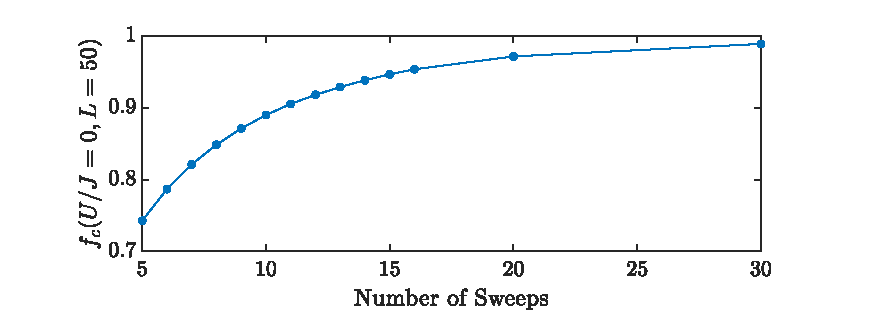
\includegraphics[width=0.9\textwidth]{Figures/CFsweeps.pdf}
    \caption{Condensate fraction as a function of number of sweeps of the DMRG algorithm in the superfluid limit. A max bond dimension of $D = 250$ was used.}
    \label{fig:sweepdependence}
\end{figure}

In \cite{Kuhner2000} the critical point of the phase transition between the superfluid and Mott-insulator was determined as $\left( {U}/{J} \right)_{crit} = 3.37$ by examining the correlations of the system. Alternatively, one could determine the critical point through the condensate fraction. In the thermodynamic limit one would expect the condensate fraction to drop to zero, as the critical point is reached (as observed in 2D by \cite{Spielman2008}).
Due to the finite system-sizes examined here, no such sharp indication of a phase transition is present in figure \ref{fig:CondensateFraction}(a). Nevertheless, the condensate fraction does appear to decrease faster around $U/J \approx 4$. As this decrease becomes more pronounced for larger systems, it is reasonable to conclude from figure \ref{fig:CondensateFraction}(a) that $\left( {U}/{J} \right)_{crit} \in [ 2.5 , 5 ]$. While this is not an exact position of the critical point, it is already a much better approximation than the mean-field result of $\left( U/J \right)_{crit}^{MF} = 11.66$ derived in Section \ref{sec:MeanFieldDiagram}.


\subsubsection{Single-particle correlations of the superfluid and Mott-insulator phases}

Correlation functions can be used to characterize quantum systems. Single-particle correlations decay exponentially in a Mott-insulator, while they for superfluids decay following a power-law 
\begin{equation}
	\braket{\hat{a}_{i}^{\dag} \hat{a}_{j}} \sim |i - j|^{-K_b /2} \; ,
	\label{eq:superfluidCorrelation}
\end{equation}
where $K_b$ is the Tomonaga-Luttinger parameter \cite{characPhases}. To illustrate the very different properties of the two Bose-Hubbard phases, the density matrices \eqref{eq:DensityMatrixEntry} for $L = 50$ and $U/J = 0, \; 0.5, \; 12$ were calculated using ground states obtained through the DMRG algorithm. 
\begin{figure}[h!]
    \centering
    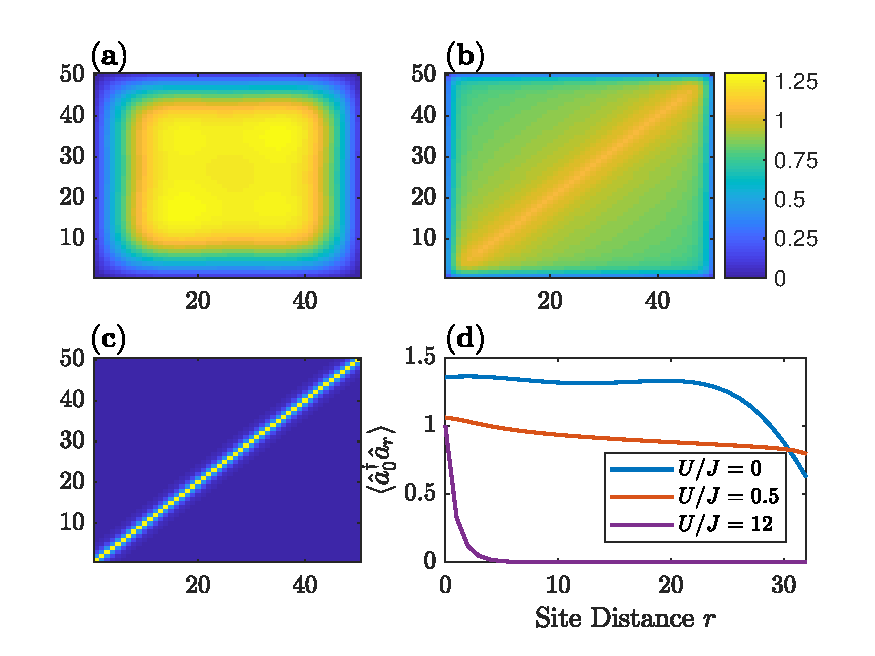
\includegraphics[width=0.9\textwidth]{Figures/DensityMatrices.pdf}
    \caption{Density matrices \eqref{eq:DensityMatrixEntry} of a 50 site system for \textbf{(a)} $U/J = 0$, \textbf{(b)} $U/J = 0.5$, and \textbf{(c)} $U/J = 12$. \textbf{(d)} Single-particle correlation function extracted from the entries of the 15th row of the density matrices. The correlations are plotted as a function of distance from the diagonal, $r$. }
    \label{fig:DensityMatrices}
\end{figure}

Figure \ref{fig:DensityMatrices}(a) shows the density matrix in the superfluid limit $U/J = 0$. In the superfluid phase, the energy of the system is minimized by de-localizing the particles across the entire lattice, whereby the atoms are essentially described by Bloch waves. Therefore, the single-particle correlations, $\bra{\psi} \hat{a}_{i}^{\dag} \hat{a}_{j} \ket{\psi}$, are very long-ranged. However, due to the open boundary conditions, particles can only tunnel in one direction at the outer sites, which effectively causes a depletion of their population. This can be seen from the diagonal of the density matrix, which describes the population at each site as
\begin{equation}
	\bra{\psi} \hat{a}_{i}^{\dag} \hat{a}_{i} \ket{\psi} = \braket{\psi | \hat{n}_i | \psi} \; .
\end{equation}
The depletion of population at the outer sites causes the single-particle correlations to exhibit a sharp decrease near the edges of the system.

Meanwhile, figure \ref{fig:DensityMatrices}(b) illustrates the density matrix for $U/J = 0.5$. The ground state is still in the superfluid phase, but the system now has finite interactions. The finite interactions causes the atoms to no longer condense into a single momentum state. The resulting spread in momentum-space causes the atoms no longer be completely de-localized in real-space, which is noticeable from the visible diagonal of the density matrix. The stronger localization due to interactions results in a much smaller effect of boundary conditions compared to the non-interacting case. 

Finally, the density matrix plotted in figure \ref{fig:DensityMatrices}(c) belongs to a system in the Mott-insulating regime. Here, the particles are highly localized, which is apparent from the dominating diagonal elements. Furthermore, in the Mott-insulator limit, interactions between sites are highly suppressed, whereby the single-particle correlations decay exponentially. For ground states even deeper in the Mott regime, the correlations would be even further suppressed, whereby the correlation length would decrease to even fewer sites. 

To quantitatively compare the correlations of the different states, the single-particle correlation functions were extracted from the density matrices. Figure \ref{fig:DensityMatrices}(d) displays the correlations as function of distance from a reference site in the lattice.
Starting with the $U/J = 0.5$ system, the ground state is clearly in the superfluid phase, as the correlations are very long-ranged and decay following a power law \eqref{eq:superfluidCorrelation}. This should also be the case in the $U/J = 0$ limit, however, the correlation function does not exhibit a power-law behavior. The reason for this is two-fold: First, correlation functions are given by an exponential series in the MPS representation, which causes a poor description of very long-ranged correlation. This is further elaborated in Appendix \ref{sec:CorrelationLength}. Secondly, in the limit of large systems and negligible interactions the superfluid spectrum becomes gapless, whereby the DMRG algorithm fails to find the exact ground state. Finally, the correlation function for the $U/J = 12$ state is clearly exponential, thereby confirming that the state is indeed in the Mott-insulator phase.



\section{Time Evolution of Matrix Product States}
Several algorithms for time evolving matrix product states exist, however, they all origin from the same ideas proposed in \cite{Vidal2003,Vidal2004}. The most widely used of these algorithms is the tDMRG algorithm \cite{Daley2004}, which gets its name from its similarity with the ground state search algorithm described in section \ref{sec:DMRG}. The tDMRG algorithm has been utilized in several instances to simulate the dynamics of one-dimensional systems \cite{Verstraete2004,Vznidarivc2008,Cazalilla2002}, and it has even been previously used in conjunction with the CRAB algorithm to perform optimal control of the superfluid to Mott-insulator phase transition \cite{FrankBloch,Doria2011}.

Although the standard algorithms for time evolution are quite efficient, further improvements can be made to the algorithms by tailoring them to the problem at hand. Therefore, a modified version of the tDMRG algorithm is proposed in Section \ref{sec:modTMDRG}, which directly utilizes the properties of the Bose-Hubbard Hamiltonian.


\subsection{The tDMRG Algorithm}
Consider the time evolution of a quantum state
\begin{equation}
	\ket{\psi (t)} = \hat{\mathcal{U}}(t) \ket{\psi (0)} \; ,
\end{equation}
where $\hat{\mathcal{U}}(t) = \e^{ - \im \hat{H} t }$ is the time evolution operator. 
Time evolution of matrix product states is similarly to the ground state search, as the bonds between the tensors are evolved rather than the tensors themselves \cite{Vidal2003,Vidal2004}. Thus, the time evolution operator must be decomposed into two-site tensors. The simplest realization of this is achieved by considering a Hamiltonian containing only nearest-neighbour interactions.
Assume the Hamiltonian is a sum of two-site operators of the form $\hat{H} = \sum_{n} \hat{h}^{[n , n+1]}$. One can decompose this into a sum over even and odd bonds \cite{Vidal2004}
\begin{equation}
	\hat{H} = \hat{H}_{\mathrm{odd}} \; + \; \hat{H}_{\mathrm{even}} = \sum_{n \; \mathrm{odd}} \hat{h}^{[n , n+1]} \; + \; \sum_{n \; \mathrm{even}} \hat{h}^{[n , n+1]} \; .
\end{equation}  
Exponentiating the Hamiltonian is non-trivial due to the non-commutativity of the operators
\begin{equation}
	[ \hat{h}_{\mathrm{odd}}^{[n , n+1]} \; , \; \hat{h}_{\mathrm{even}}^{[n , n+1]} ] \neq 0 \; .
\end{equation}
Considering a small time slice, $\Delta t$, the exponentiation can be achieved through the Trotter-Suzuki expansion \cite{Suzuki1991}. To first order this reads
\begin{equation}
	\e^{- \im \hat{H} \; \Delta t} = \e^{- \im \hat{H}_{\mathrm{odd}} \; \Delta t } \e^{- \im \hat{H}_{\mathrm{even}} \; \Delta t} \; + \; \;  \mathrm{O}(\Delta t^2) \; ,
\end{equation}
where the error is due to the non-commutativity of the bond Hamiltonians. Thus, the time evolution operator can be expressed as the product
\begin{equation}
	\hat{\mathcal{U}}(\Delta t) \approx \left( \prod_{n \; \mathrm{odd}} \hat{\mathcal{U}}^{[n,n+1]} (\Delta t) \right) \left( \prod_{n \; \mathrm{even}} \hat{\mathcal{U}}^{[n,n+1]} (\Delta t) \right) \; , \label{eq:SuzukiTrotter1stOrder}
\end{equation}
where
\begin{equation}
	\hat{\mathcal{U}}^{[n,n+1]} (\Delta t) = \e^{- \im \hat{h}^{[n , n+1]} \; \Delta t } \; .
\end{equation}
The result is an MPO performing an infinitesimal time step on the odd bonds, and another MPO evolving the even bonds. An illustration of eq. \eqref{eq:SuzukiTrotter1stOrder} is shown in Figure \ref{fig:oddevenops}.
\begin{figure}[b]
	\centering
	\begin{tikzpicture}[inner sep=1mm]
	\def \reldist {1.5};
	\def \numb {6};
	\def \wid {2}

	\foreach \i in  {1,...,\numb} {
		\node[tensor] (t\i) at (\i * \reldist, 0) {};
		\draw[-] (t\i) -- (\i * \reldist , -2.8);	
	};
	
	\foreach \i in {1,...,5} {
        \pgfmathtruncatemacro{\iplusone}{\i + 1};
        \draw[-] (t\i) -- (t\iplusone);
	};
	
	\foreach \i in {1,3,5} {
        \node[twositeop, minimum width= \wid cm] (op\i) at (\reldist*\i + \wid/2 -0.25,-1) {$\hat{\mathcal{U}}^{\mathrm{even}} (\Delta t)$};
	};
	
	\foreach \i in {2,4,6} {
        \node[twositeop, minimum width= \wid cm] (op\i) at (\reldist*\i + \wid/2 -0.25,-2) {$\hat{\mathcal{U}}^{\mathrm{odd}} (\Delta t)$};
	};	
	
	\node (dot1) at (0,0) {$\dots$};
	\node (dot2) at (\numb * \reldist + \reldist,0) {$\dots$};
	\draw[-] (t1) -- (dot1);
	\draw[-] (t\numb) -- (dot2);
	
	\draw[decoration={calligraphic brace,amplitude=10pt}, decorate, line width=1.25pt, xshift=-4pt, yshift=0pt]
(0, -2.5) -- (0,-0.5) node [black,midway,xshift=-1.0cm] 
{\large $\hat{\mathcal{U}} ( \Delta t)$};
	
\end{tikzpicture}
	\caption{Approximation of each time step $\Delta t$ using a Trotter-Suzuki expansion, such that the time evolution operator is expressed as a product of unitary two-site operators.}
	\label{fig:oddevenops}
\end{figure}
The tDMRG algorithm describes the most efficient and accurate way of contracting the tensor network detailed in figure \ref{fig:oddevenops}. The algorithm gets its name from its similarity with the DMRG algorithm detailed in section \ref{sec:DMRG}. In fact, the merge and unmerge procedure of the two algorithms are completely identical, whereby they only differ in the steps of applying the operator and proceeding to the next site. The following procedure details a time evolution step of the $n$'th bond \cite{schollwock}.

\subsubsection{Infinitesimal time-step update for tDMRG}
\begin{enumerate}
\item
\textbf{Merge:} Contract tensors $M^{[n]}$ and $M^{[n+1]}$ over the bond $\alpha_{n}$ creating a two-site tensor $\Theta^{j_n , j_{n+1}}$.

\item
\textbf{Apply unitary:} The two-site time evolution operator, $\hat{\mathcal{U}}^{[n, n+1]}$, is applied to $\Theta^{j_n , j_{n+1}}$
\begin{equation}
	\tilde{\Theta}_{\alpha_{n-1} , \alpha_{n+1}}^{j_n , j_{n+1} } = \sum_{j_n ', j_{n+1}'} \mathcal{U}^{j_n  j_{n+1} , j_n '  j_{n+1}'} \; \Theta_{\alpha_{n-1} , \alpha_{n+1}}^{j_n ', j_{n+1} ' } \; .
\end{equation}

\item
\textbf{Unmerge:} Reshape $\tilde{\Theta}_{\alpha_{n-1} , \alpha_{n+1}}^{j_n ', j_{n+1} '}$ to a matrix and decompose it through an SVD. Applying $\hat{\mathcal{U}}^{[n, n+1]}$ causes an increase in bond dimension, $D \rightarrow d^2 D$, which must be truncated by keeping only the $D$ largest singular values from the SVD. 

\item
\textbf{Progress:}  Next, the center cite of the MPS must be shifted by two, in order to update the next even (odd) bond. This is achieved by merging tensors $M^{[n+1]}$ and $M^{[n+2]}$ and performing a second SVD, while reshaping the resulting $U$-matrices to left-normalised tensors to retain the canonical form. The product of the second SVD must be truncated as well, however, no loss of information will occur, as the Schmidt rank of the matrix $S$ will be at most $D$ following the first SVD. 
\end{enumerate}
Following the procedure above will leave the MPS in position for application of the unitary $\hat{\mathcal{U}}^{[n+2 , n+3]}$. The efficiency of the tDMRG algorithm depends on the sequence in which bonds are evolved. A simple, yet effective way is iterating from left to right when evolving even bonds, while iterating right to left when evolving odd bonds. Thereby, the centered cite of the mixed-canonical form is moved continuously through the MPS, rather than having to be reset when reaching the end of the system.

It has been shown that the area law scaling of entanglement of an initial state will remain true even for longer times \cite{Bravyi2006,Eisert2006}. Simultaneously, the pre-factor of the area-law is expected to grow exponentially \cite{Schuch2008}. Therefore, the maximum bond dimension, $D$, kept in each iteration of the tDMRG algorithm must be chosen sufficiently high in order to properly capture the relevant dynamics of the system. Alternatively, one can truncate the bond dimensions of the tensors according to some eigenstate-contribution threshold, $\epsilon_t$. While this will ensure a consistent description of the state throughout the simulation, the bond dimension may grow very large thereby causing a significant decrease in the efficiency of the algorithm. Thus, analyzing the evolution of the bond dimension is imperative for the success of the simulation when examining phenomena of high entanglement such as phase transitions.

Although the tDMRG algorithm is a very powerful algorithm, an even higher efficiency can be achieved when tailoring the algorithm to the system - in this case the Bose-Hubbard model. Thus, the Hamiltonian contains both nearest-neighbour and on-site terms. Furthermore, the Hamiltonian is time dependent, since the lattice depth is varied when driving a phase transition, whereby the propagator at each time step is different. The following algorithm is a modification of the tDMRG algorithm, which is tailored for conducting optimal control using the Bose-Hubbard Hamiltonian.


\subsection{Modified Time Evolution Algorithm for Bose-Hubbard Model}
\label{sec:modTMDRG}
The control problem solved in this thesis consist of dynamically transferring a superfluid ground state to a Mott-insulating ground state. Thus, the Hamiltonian is time-dependent, whereby it must be exponentiated for every time-step to create the propagators required for the time-evolution. Furthermore, any optimization of the control sequence will require the corresponding propagators to be re-calculated. Thus, the computational time of the propagators must be taken into account. Typically, operators are exponentiated through series expansions, however, this is in general a rather expensive operation. Therefore, choosing control-Hamiltonians which are easy to exponentiate is often an advantage.

The phase of the Bose-Hubbard model depends on the ratio $U/J$, where $U$ is the interaction matrix element \eqref{eq:BHparamU}, and $J$ is the tunneling matrix element \eqref{eq:BHparamJ}. Both parameters are dependent of the lattice depth, which therefore has been used as control function in previous studies \cite{FrankBloch,Doria2011}. Exponentiating the tunneling Hamiltonian is non-trivial, however, the interaction Hamiltonian is diagonal, whereby the propagator can be computed by simply exponentiating the elements of the matrix. Thus, choosing the ratio $U/J$ as the control function and working in units of $J$ significantly simplifies the calculation of propagators, as the tunneling propagator remains constant. Employing a second-order Suzuki-Trotter expansion
\begin{equation}
	\exp\left( \text{-}i ( \hat{H}_J + \hat{H}_U  ) \Delta t \right) = \exp\left( \text{-} i \hat{H}_U \Delta t /2  \right) \exp\left( \text{-} i \hat{H}_J \Delta  t \right) \exp\left( \text{-} i \hat{H}_U \Delta t /2  \right) + O(\Delta t^3) \; ,
	\label{eq:SuzukiTrotter}
\end{equation}
allows separate exponentiation of the two parts of the Bose-Hubbard Hamiltonian, whereby only the interaction needs to be updated. Again, the error is due to the non-commutativity of operators. Thereby, the expanded propagator reads
\begin{equation}
	\hat{\mathcal{U}} (\Delta t) = \left( \prod_{i = 1}^{L} \hat{\mathcal{U}}_{U}^{[i]} \right) \left( \prod_{i \; \mathrm{odd}}^{L} \hat{\mathcal{U}}_{J}^{[i,i+1]}  \right) \left( \prod_{i \; \mathrm{even}}^{L} \hat{\mathcal{U}}_{J}^{[i,i+1]}  \right) \left( \prod_{i = 1}^{L} \hat{\mathcal{U}}_{U}^{[i]} \right) \; ,
\end{equation}
where the site-specific propagators, or gates, are given by
\begin{align}
	\hat{\mathcal{U}}_{J}^{[i,i+1]} &= \exp \left( \text{-} i J ( \hat{a}_{i}^{\dag} \hat{a}_{i+1} + \hat{a}_{i+1}^{\dag} \hat{a}_{i} ) \Delta t \right) \\
	\hat{\mathcal{U}}_{U}^{[i]} &= \exp \left( \text{-} i \frac{U}{2} \hat{n}_i (\hat{n}_i -1) \Delta t /2 \right) \; .
\end{align}
\begin{figure}[h!]
	\centering
	\begin{tikzpicture}[inner sep=1mm]
\def \reldist {2};
\def \numb {4};
\def \wid {2.8};
\def \size {1.0};
\def \hi {0.8};
\def \vert {1.25};
\def \rad {0.4};

	
\foreach \i in  {1,...,\numb} {
	\node[tensor,minimum width= \size cm,minimum height= \size cm, rounded corners = 0.2cm] (A\i)
	at (\i * \reldist, 0) {$M^{[ \i ]}$};
	\draw[-] (A\i) -- (\i * \reldist , -4.7*\vert);	
};

\foreach \i in {1,...,3} {
    \pgfmathtruncatemacro{\iplusone}{\i + 1};
    \draw[-] (A\i) -- (A\iplusone);
};


\foreach \i in  {1,...,\numb} {
	\node[operator,minimum width= \hi cm,minimum height= \hi cm] (op\i)
	at (\i * \reldist, -\vert )
	{\scriptsize $\hat{\mathcal{U}}_{U}^{[ \i ]}$};	
};

\foreach \i in {1,...,\numb} {
	\pgfmathtruncatemacro{\j}{\i + 1};
    \node[twositeop, minimum width= \wid cm,minimum height= \hi cm,rounded corners = \rad cm] (eop\i)
    at (\reldist*\i + \reldist/2, {-2*\vert - Mod(\j,2) *\vert })
    {\small $\hat{\mathcal{U}}_{J}^{[ \i , \j ]} $};
};

\foreach \i in  {1,...,\numb} {
	\node[operator,minimum width= \hi cm,minimum height= \hi cm] (op\i)
	at (\i * \reldist, -4*\vert )
	{\scriptsize $\hat{\mathcal{U}}_{U}^{[ \i ]}$};	
};




\draw[decoration={calligraphic brace,amplitude=10pt}, decorate, line width=1.25pt, xshift=-4pt, yshift=0pt]
(0.5, -4*\vert -0.4) -- (0.5,-0.8) node [black,midway,xshift=-1.0cm] 
{\large $\hat{\mathcal{U}} ( \Delta t)$};


\draw[decoration={calligraphic brace,amplitude=10pt,mirror}, decorate, line width=1.25pt, xshift=-4pt, yshift=0pt]
(\numb * \reldist + 3, -2*\vert -0.5) -- (\numb * \reldist + 3,-0.8) node [black,midway,xshift=1.2cm] 
{\normalsize \begin{tabular}{c}
				$\rightarrow$ \\
				Sweep \\
			  \end{tabular} };


\draw[decoration={calligraphic brace,amplitude=10pt,mirror}, decorate, line width=1.25pt, xshift=-4pt, yshift=0pt]
(\numb * \reldist + 3, -4*\vert -0.4) -- (\numb * \reldist + 3,-2*\vert -0.6) node [black,midway,xshift=1.2cm] 
{\normalsize \begin{tabular}{c}
				$\leftarrow$ \\
				Sweep \\
			  \end{tabular} };


\node (dot2) at (\numb * \reldist + 2,0) {$\dots$};
\draw[-] (A\numb) -- (dot2);
	
	
\end{tikzpicture}
	\caption{Tensor diagram depicting a single time step of the modified tDMRG algorithm. The tensors of the upper part of the network are contracted with the MPS while sweeping from left to right, whereas the lower part is applied with a right-to-left sweep.}
	\label{fig:ModifiedTEBD}
\end{figure}
A single time step, $\Delta t$, using the expanded operator is represented diagrammatically in figure \ref{fig:ModifiedTEBD}. At first glance, the tensor network resulting from the Suzuki-Trotter expansion may seem rather extensive, however, it can be contracted in a very efficient manner. The upper part of the network is contracted in a left-to-right sweeping manner, where the position of the center cite, and thereby the normalization of the MPS, is pushed to the right following each step. Likewise, the lower part of the network is contracted though a right-to-left sweep such that the MPS returns to its original form centered on the first site after applying the final operator. Thereby, the MPS is immediately ready for the subsequent time-propagation.

The sequence of contractions of the left-to-right sweep is shown in figure \ref{fig:TEBDContraction}. The MPS is initially centered on the first tensor, while its remaining tensors are right-normalised. By contracting the bonds marked with a bold line shown in step 1 and 2, the operators are efficiently applied to the MPS. In the third step, the two-site tensor, $\Theta$, is split using an SVD, where the bond dimension of the tensors is truncated. This is crucial in order to maintain a reduced dimensionality, which would otherwise result in a significant increase in contraction time. In the final and fourth step, the central cite of the MPS is moved to the start of the next two-site operator through another site merge and subsequent SVD. This step is exactly as in the original tDMRG algorithm. Thereby the normalization of the MPS is "pushed" to the right and contained in a single site, which makes it easy to deal with in the end of the time evolution step.

\begin{figure}[t!]
\centering % <-- add this
\begin{subfigure}[b]{0.4\textwidth}
	\caption{}  
  	\begin{tikzpicture}[inner sep=1mm]
\def \reldist {1.5};
\def \numb {4};
\def \wid {2.3};
\def \size {1.0};
\def \hi {0.8};
\def \rad {0.4};
\def \vert {1.35};


\foreach \i in  {1,...,\numb} {
	\node[tensorr,minimum width= \size cm,minimum height= \size cm, rounded corners = 0.2cm] (A\i)
	at (\i * \reldist, 0) {$M^{[ \i ]}$};
	\draw[-] (A\i) -- (\i * \reldist , -2.5*\vert);	
};

\foreach \i in {1,...,3} {
    \pgfmathtruncatemacro{\iplusone}{\i + 1};
    \draw[-] (A\i) -- (A\iplusone);
};

\node[tensorc,minimum width= \size cm,minimum height= \size cm, rounded corners = 0.2cm] (C) at (1 * \reldist, 0) {$M^{[1]}$};


\foreach \i in  {1,...,\numb} {
	\draw[-] (A\i) -- (\i * \reldist , -2.6 *\vert);	
};

\draw[-,line width=0.8mm] (A1) -- (A2);

\foreach \i in  {1,...,\numb} {
	\node[operator,minimum width= \hi cm,minimum height= \hi cm] (op\i)
	at (\i * \reldist, -\vert)
	{\scriptsize $\hat{\mathcal{U}}_{U}^{[ \i ]}$};	
};

\foreach \i in {1,3} {
	\pgfmathtruncatemacro{\j}{\i + 1};
    \node[twositeop, minimum width= \wid cm,minimum height= \hi cm,rounded corners = \rad cm] (top\i)
    at (\reldist*\i + \reldist/2, -2*\vert)
    {\small $\hat{\mathcal{U}}_{J}^{[ \i , \j ]} $};
};


\node (dot2) at (\numb * \reldist + 1.4,0) {$\dots$};
\draw[-] (A\numb) -- (dot2);
	
	
\end{tikzpicture}
\end{subfigure}
\hspace{10mm}
\begin{subfigure}[b]{0.4\textwidth}
	\caption{}    
  	\begin{tikzpicture}[inner sep=1mm]
\def \reldist {1.5};
\def \numb {4};
\def \wid {2.3};
\def \size {1.0};
\def \hi {0.8};
\def \rad {0.4};
\def \vert {1.35};


\foreach \i in  {1,...,\numb} {
	\node[operator] (A\i)
	at (\i * \reldist, 0) {};
	\draw[-] (A\i) -- (\i * \reldist , -2.5*\vert);	
};

\foreach \i in {1,...,3} {
    \pgfmathtruncatemacro{\iplusone}{\i + 1};
    \draw[-] (A\i) -- (A\iplusone);
};


\foreach \i in  {1,...,\numb} {
	\draw[-] (A\i) -- (\i * \reldist , -2.6 *\vert);	
};

\node[operator] (d1) at (1 * \reldist, -\vert) {};
\node[operator] (d2) at (2 * \reldist, -\vert) {};
\node[operator] (dd1) at (1 * \reldist, -2*\vert) {};
\node[operator] (dd2) at (2 * \reldist, -2*\vert) {};


\draw[-,line width=0.8mm] (A1) -- (d1);
\draw[-,line width=0.8mm] (A2) -- (d2);
\draw[-,line width=0.8mm] (dd1) -- (d1);
\draw[-,line width=0.8mm] (dd2) -- (d2);

\foreach \i in  {1,...,\numb} {
	\node[operator,minimum width= \hi cm,minimum height= \hi cm] (op\i)
	at (\i * \reldist, -\vert)
	{\scriptsize $\hat{\mathcal{U}}_{U}^{[ \i ]}$};	
};

\foreach \i in {1,3} {
	\pgfmathtruncatemacro{\j}{\i + 1};
    \node[twositeop, minimum width= \wid cm,minimum height= \hi cm,rounded corners = \rad cm] (top\i)
    at (\reldist*\i + \reldist/2, -2*\vert)
    {\small $\hat{\mathcal{U}}_{J}^{[ \i , \j ]} $};
};


\node (dot2) at (\numb * \reldist + 1.4,0) {$\dots$};
\draw[-] (A\numb) -- (dot2);

\foreach \i in  {3,...,\numb} {
	\node[tensorr,minimum width= \size cm,minimum height= \size cm, rounded corners = 0.2cm] (B\i)
	at (\i * \reldist, 0) {$M^{[ \i ]}$};
};
\node[tensor,minimum width= \wid cm,minimum height= \size cm, rounded corners = 0.2cm] (AA) at (\reldist*1 + \reldist/2, 0) {\Large $\Theta$};



	\node (node1) at (\reldist +0.2, -0.5*\vert -0.05) {\small \textbf{1}};
	\node (node2) at (2*\reldist +0.2, -0.5*\vert -0.05) {\textbf{1}};
	\node (node3) at (\reldist +0.2, -1.5*\vert) {\textbf{2}};
	\node (node4) at (2*\reldist +0.2, -1.5*\vert) {\textbf{2}};	
	
\end{tikzpicture}
\end{subfigure}
\\ % <-- add this
\vspace{5mm}
\begin{subfigure}[b]{0.4\textwidth}
	\caption{}    	
  	\begin{tikzpicture}[inner sep=1mm]
\def \reldist {1.5};
\def \numb {4};
\def \wid {2.3};
\def \size {1.0};
\def \hi {0.8};
\def \rad {0.4};
\def \vert {1.35};


\foreach \i in  {1,...,\numb} {
	\node[tensorr,minimum width= \size cm,minimum height= \size cm, rounded corners = 0.2cm] (A\i)
	at (\i * \reldist, 0) {$M^{[ \i ]}$};
	\draw[-] (A\i) -- (\i * \reldist , -2.5*\vert);	
};

\foreach \i in {1,...,3} {
    \pgfmathtruncatemacro{\iplusone}{\i + 1};
    \draw[-] (A\i) -- (A\iplusone);
};

\node[tensorl,minimum width= \size cm,minimum height= \size cm, rounded corners = 0.2cm] (L) at (1 * \reldist, 0) {$M^{[1]}$};

\node[tensorc,minimum width= \size cm,minimum height= \size cm, rounded corners = 0.2cm] (C) at (2 * \reldist, 0) {$M^{[2]}$};


\foreach \i in  {1,...,\numb} {
	\draw[-] (A\i) -- (\i * \reldist , -2.6 *\vert);	
};

\draw[-,line width=0.8mm] (A2) -- (A3);

\foreach \i in  {3,...,\numb} {
	\node[operator,minimum width= \hi cm,minimum height= \hi cm] (op\i)
	at (\i * \reldist, -\vert)
	{\scriptsize $\hat{\mathcal{U}}_{U}^{[ \i ]}$};	
};

\foreach \i in {3} {
	\pgfmathtruncatemacro{\j}{\i + 1};
    \node[twositeop, minimum width= \wid cm,minimum height= \hi cm,rounded corners = \rad cm] (top\i)
    at (\reldist*\i + \reldist/2, -2*\vert)
    {\small $\hat{\mathcal{U}}_{J}^{[ \i , \j ]} $};
};


\node (dot2) at (\numb * \reldist + 1.4,0) {$\dots$};
\draw[-] (A\numb) -- (dot2);
	
	
\end{tikzpicture}
\end{subfigure}
\hspace{10mm}
\begin{subfigure}[b]{0.4\textwidth}
	\caption{}  
  	\begin{tikzpicture}[inner sep=1mm]
\def \reldist {1.5};
\def \numb {4};
\def \wid {2.3};
\def \size {1.0};
\def \hi {0.8};
\def \rad {0.4};
\def \vert {1.35};


\foreach \i in  {1,...,\numb} {
	\node[tensorr,minimum width= \size cm,minimum height= \size cm, rounded corners = 0.2cm] (A\i)
	at (\i * \reldist, 0) {$M^{[ \i ]}$};
	\draw[-] (A\i) -- (\i * \reldist , -2.5*\vert);	
};

\foreach \i in {1,...,3} {
    \pgfmathtruncatemacro{\iplusone}{\i + 1};
    \draw[-] (A\i) -- (A\iplusone);
};

\node[tensorl,minimum width= \size cm,minimum height= \size cm, rounded corners = 0.2cm] (L1) at (1 * \reldist, 0) {$M^{[1]}$};

\node[tensorl,minimum width= \size cm,minimum height= \size cm, rounded corners = 0.2cm] (L2) at (2 * \reldist, 0) {$M^{[2]}$};

\node[tensorc,minimum width= \size cm,minimum height= \size cm, rounded corners = 0.2cm] (C) at (3 * \reldist, 0) {$M^{[3]}$};


\foreach \i in  {1,...,\numb} {
	\draw[-] (A\i) -- (\i * \reldist , -2.6 *\vert);	
};

\draw[-,line width=0.8mm] (A3) -- (A4);

\foreach \i in  {3,...,\numb} {
	\node[operator,minimum width= \hi cm,minimum height= \hi cm] (op\i)
	at (\i * \reldist, -\vert)
	{\scriptsize $\hat{\mathcal{U}}_{U}^{[ \i ]}$};	
};

\foreach \i in {3} {
	\pgfmathtruncatemacro{\j}{\i + 1};
    \node[twositeop, minimum width= \wid cm,minimum height= \hi cm,rounded corners = \rad cm] (top\i)
    at (\reldist*\i + \reldist/2, -2*\vert)
    {\small $\hat{\mathcal{U}}_{J}^{[ \i , \j ]} $};
};


\node (dot2) at (\numb * \reldist + 1.4,0) {$\dots$};
\draw[-] (A\numb) -- (dot2);
	
	
\end{tikzpicture}
\end{subfigure}
\caption{\textit{Sequence of contractions for modified tDMRG algorithm during left to right sweep. Step \textbf{(1)}: MPS is centered on site 1. Tensors $M^{[1]}$ and $M^{[2]}$ are contracted. Step \textbf{(2)}: Two-site tensor, $\Theta$, is contracted with operators in numbered sequence. The propagated two-site tensor is split using an SVD in step \textbf{(3)}, followed by a contraction to the right. Lastly, in step \textbf{(4)}, the two-site tensor of $M^{[2]}$ and $M^{[3]}$ is split using another SVD, whereby the center (and thereby the normalisation) is pushed to site 3.}}
\label{fig:TEBDContraction}
\end{figure}
As the center reaches the end of the MPS, the direction of the sweep is reversed. The right-to-left sweep is very similar to the sequence described above. The main difference is in the order of contractions, as the $\hat{\mathcal{U}}_{J}^{[i,i+1]}$-propagator is applied before $\hat{\mathcal{U}}_{U}^{[i]}$. As the sweep, and thereby the central cite, reaches the first site of the MPS, the central site is divided by its norm. Thereby the MPS is normalized and in the same configuration as before the time step. Thus, further propagations can be performed readily.

Additional precision is achieved when evaluating the control at the beginning and end points of the time interval \cite{Steck2007}. Thus, the left-to-right sweep applies the operator $\hat{\mathcal{U}}_{U(t)}^{[i]} $, while the right-to-left sweep applies $\hat{\mathcal{U}}_{U(t + \Delta t)}^{[i]}$.

The time-evolution algorithm described here shares many traits with one proposed in \cite{Daley2004}, which was tested on the Bose-Hubbard model. The algorithm displayed weak convergence with the maximum bond dimension, $D$, whereby precise results can be obtained using only small bond dimensions. Further improvements to the method were suggested in \cite{Daley2004}, which included utilizing even higher-order expansions of the propagator. By evaluating the parameters of the propagator at specific points in the time interval, $\Delta t$, many algorithmic sweeps can be combined, greatly reducing the computational cost \cite{Yoshida1990,Krech1998}.


\subsubsection{Time complexity of time-evolution algorithms}
\begin{figure}[h!]
    \centering
    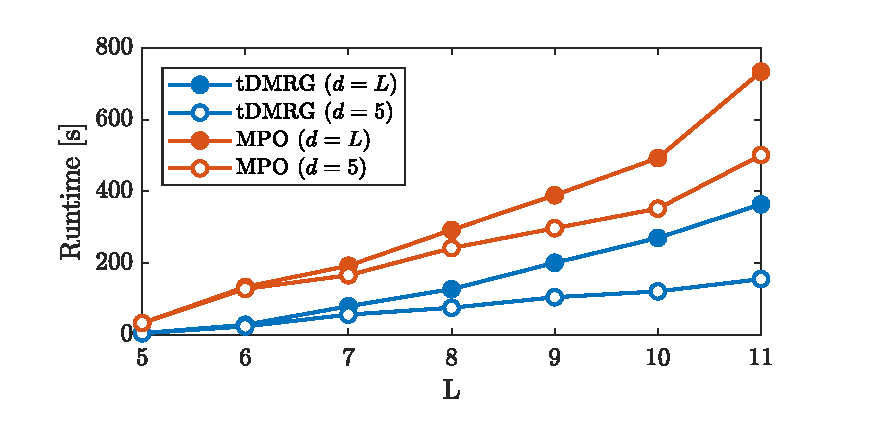
\includegraphics[width=0.8\textwidth]{Figures/CompareRuntime.pdf}
    \caption{Runtime of propagating 100 time steps in a Bose-Hubbard system with unit occupancy using two different algorithms. The filled data point were calculated for tensors with physical dimension, $d$, equal to the lattice size, $L$, while the physical dimension was set to a constant $d = 5$ for the empty points. }
    \label{fig:CompareRuntime}
\end{figure}
Figure \ref{fig:CompareRuntime} compares runtimes between the modified tDMRG algorithm and the default time evolution method of the ITensor library \cite{ITensor}. The two methods were compared for various lattice sizes with unit occupancy. The default ITensor method builds the entire propagator as a single layer MPO following \cite{Pollmann2015}. Afterwards, the MPO is applied to the MPS according to eq. \eqref{eq:optBracketsMPO}. The two methods were tested for both local Fock space dimensions equal to the length of the lattice, $d = L$, and a truncation of the Fock space at a constant value of $d = 5$.
Clearly, the modified tDMRG algorithm outperforms the library method by a large margin. In fact, for large systems it is about twice as fast for both dimensions of the Fock space.

In Section \ref{sec:MPO} the cost of applying an MPO to an MPS was given by $\mathcal{O}(L d^2 D_W ^2 D^2)$. Since the tDMRG propagator consists of multiple gates rather than a connected layer, the operator bond dimension, $D_W$, is unit. Thus, the tDMRG algorithm has a cubic scaling with system size. The MPO-approach is slower due to $D_W$ being larger than unit. However, the operator bond dimension is independent of the system size for the Bose-Hubbard model. Therefore, the MPO-algorithm should also exhibit cubic scaling with system size, although with a larger pre-factor than the tDMRG algorithm. Examining figure \ref{fig:CompareRuntime}, the cubic scaling of the $d = L$ calculations is not completely obvious at small system sizes, although the scaling does not appear linear. Had even larger systems been examined, the cubic scaling would have been more apparent.

A much better scaling can be achieved by truncating the local Hilbert space such that $d$ is kept constant. Doing so should result in a runtime scaling linearly with the system size. The linear scaling clearly applies for the modified tDMRG algorithm in figure \ref{fig:CompareRuntime}. Therefore, truncating the physical of the MPS should enable efficient simulations of large lattice system. However, performing such a truncation implies discarding states corresponding to a high occupation at a single site from the Hilbert space.
In the case of the Bose Hubbard model, eq. \eqref{BHhamil}, the interaction term scales quadratically with the number of particles at a given site. Thus, having multiple particle occupying the same site is accompanied by a huge increase in energy. Such high energy states are very hard to reach in large systems, whereby neglecting contributions from states with a majority of the particles at a single site is a reasonable approximation \cite{Daley2004}.

Therefore, the modified tDMRG algorithm can be applied efficiently to very large systems, if the dimension of the physical index of the MPS is restricted to a reasonable fraction of the number of particles. A similar practice was reported in \cite{Braun2015}, where Bose-Hubbard systems of various sizes were simulated. The study utilized a maximum occupation of 6 was used for lattices up to 40 sites with unit occupation. Hence, a majority of the local Fock states can be discarded without any noticeable effect on the dynamics of the overall system.